\paragraph{}{
	L'Unité Arithmétique et Logique, abrégé UAL, permet de faire des calculs
	basiques (additions, divisions, décalages de bits, etc.). Elle effectue
	les calculs sur huit bits. L'UAL a trois entrées. La première sur trois bits
	permet de préciser le code de l'opération à utiliser. Les deux autres entrées
	sur huit bits sont les opérantes de l'opération. \newline
	En sortie, sur \textit{ouput} on peut lire le résultat de l'opération. Il
	y a également quatre drapeaux comme détaillés ci-dessous.
}

\begin{itemize}
	\item[CF] pour \textit{Carrie Flag} est le drapeau levé lorsque que l'opération
	génère une retenue.
	\item[ZF] pour \textit{Zero Flag} est armé lorsque que le résultat comporte uniquement
	des $0$.
	\item[OF] pour \textit{Overflow Flag} est un drapeau levé lorsque on dépasse
	la capacité des nombres représentable par la machine.
	\item[SF] pour \textit{Sign Flag} est levé lorsque le résultat a son
	bit de poids fort à $1$, c'est un nombre signé.
\end{itemize}

\begin{figure}
	\centering
	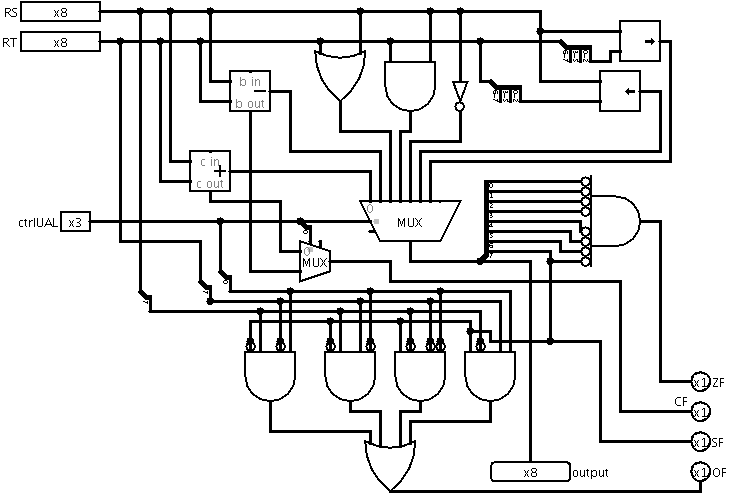
\includegraphics[scale=0.4,origin=c]{circuits/UAL.png}
	\caption{
		\label{ual_circ}
		Sch\'{e}ma \'{e}lectronique de l'Unit\'{e} Arithm\'{e}tique et Logique
	}
\end{figure}

\begin{figure}
	\centering
	\begin{tabular}{|c|c|c|c|c|}
	\hline \backslashbox{$s_{1}e_{1}$}{$e_ {2}b_{1}$} & $00$ & $00$ & $11$ & $10$ \\ 
	\hline $00$ & $0$ & $0$ & $0$ & $0$ \\ 
	\hline $01$ & $0$ & $1$ & $0$ & $1$ \\ 
	\hline $11$ & $0$ & $0$ & $0$ & $0$ \\ 
	\hline $10$ & $1$ & $0$ & $1$ & $0$ \\ 
	\hline 
	\end{tabular}
	\caption{
		\label{of_karnaugh}
		Tableau de \textsc{Karnaugh} pour le drapeau \textit{OF}
	}
\end{figure}

\paragraph{\textit{Overflow Flag}}{
	Pour armer le drapeau \textit{OF}, on fait le tableau \textsc{Karnaugh}
	de la figure \ref{of_karnaugh} d'où on tire l'équation \ref{of_equa}.
	Ainsi on peut faire facilement le circuit qui contrôle la levée du drapeau. 
}
	\begin{equation}
		\label{of_equa}
		{OF} = \neg s_{1} ( e_{1} ( \neg e_{2} . b_{1} + e_{1} . \neg b_{1} ) ) 
			+ s_{1} ( \neg e_{1} ( \neg e_{2} . \neg b_{1} + e_{2} . b_{1} ))
	\end{equation}

\paragraph{}{
	Dans l'équation \ref{of_equa}, les variables  $e_{1}$ et $e_{2}$ correspondent aux 
	bits de poids fort de \textit{Rs} et \textit{Rt}. Les variables $s_{1}$ et $b_{1}$
	correspondent respectivement au bit de poids fort du résultats de l'UAL et 
	le bit de poids faible de \textit{ctrlUAL}. On choisi ces bits car
	ils nous renseignent sur la nature du résultat. Par exemple lorsqu'on soustrait un 
	nombre négative et un nombre positif, si le résultat est positive, c'est qu'un 
	\textit{overflow} est survenu.
	
}